\documentclass[ignorenonframetext]{beamer}
%\documentclass[a4paper,12pt,titlepage]{article}
%\usepackage{beamerarticle}

\usepackage{graphicx}
\usepackage[utf8]{inputenc}
\usepackage{pdfpages}
\usepackage{textcomp}
\usepackage{fancyhdr,url}
\usepackage{amsmath}
\usepackage{mathtools}
\usepackage{Exercise}
\usepackage{tikz}
\usetikzlibrary{mindmap,datavisualization,shapes,arrows}
\usepackage{smartdiagram}
\usepackage{overpic}
\usepackage[version=4]{mhchem}
\usepackage{xcolor}
\usepackage{pgfplots}
\usepackage{subcaption}
\usepackage{float}
\setlength{\headheight}{15pt}
\setlength{\parindent}{0in}
\setlength{\parskip}{1em}

\pgfplotsset{width=\textwidth,compat=1.9}

\mode<presentation>{
\usetheme{CambridgeUS}
\AtBeginLecture{\frame{\Large Lecture: \insertlecture}}
\usepackage[absolute,overlay]{textpos}
%\includeonlylecture{Lecture 1}
%\includeonlyframes{current}
}

\logo{\includegraphics[height=1cm]{../../graphics/crac}}


\mode<article>{
\usepackage[absolute]{textpos} 
\usepackage[a4paper, top=1.5in]{geometry}
\pagestyle{fancy}
\fancyhf{}
\lhead{CM4020/CM6014}
\chead{\footnotesize Surface Science and Analysis}
\rhead{\thepage}
\lfoot{School of Chemistry, UCC}
\cfoot{\tiny{version 2022.01}}
\rfoot{Semester 2 2021/2022}}

\title{CM4020 -- Interfaces, Spectroscopy and Modelling\\
CM6014 -- Materials, Pharmaceutical and Bioanalysis}
\subtitle{\vspace{1in}\includegraphics[height=3cm]{../../graphics/M31_001}}
\author{Surface Science and Analysis \mode<article>{\vspace{1cm}\\\includegraphics[height=2cm]{../../graphics/crac}}}
\institute{School of Chemistry \\ University College Cork}
\date{Semester 2 2021/2022}

\renewcommand*\contentsname{}

\tikzset{
    invisible/.style={opacity=0},
    visible on/.style={alt={#1{}{invisible}}},
    alt/.code args={<#1>#2#3}{%
      \alt<#1>{\pgfkeysalso{#2}}{\pgfkeysalso{#3}} % \pgfkeysalso doesn't change the path
    },
  }


\begin{document}
\mode<article>{\maketitle \tableofcontents}

\begin{frame}
	\titlepage
\end{frame}

\newpage

\section*{Scope of this document}
This document contains material relevant to the surface science and analysis question of the CM4020 and CM6014 Exams, \emph{including} directed study material. 

This document is mandatory reading, along with lecture slides. 

The problems and exercises at the end will help prepare you for the exam questions, so make sure you can solve them.

\part{Surfaces, adsorption and catalysis}

\lecture{Introduction and Concepts}{Lecture 1}

\section{Surfaces}

\begin{frame}
A material surface has several physical features; there are edges, defects, holes, layers, etc.

It also has chemical properties; there are atoms and chemical groups exposed on the surface, some have ``dangling bonds'' with chemical groups attached to surface atoms, it has reactive sites and it is not usually clean, on a molecular level. 

A surface can be structured or irregular, both on an atomic scale and macroscale.
If there is no ordering in the solid state we call it \textit{amorphous}. If the atomic structure repeats itself in all directions we call it a \textit{single crystal}. A solid can also be \textit{polycrystalline} -- when there are many individual grains, each consisting of single crystal.

\begin{center} \includegraphics[width=.5\textwidth]{../../graphics/solidstructures} \end{center}
\end{frame} 

\subsection{Single crystals}


The structure of a crystalline solid, whether a metal or not, is best described by considering its simplest repeating unit, which is referred to as its unit cell.
The unit cell consists of lattice points that represent the locations of atoms or ions.
The entire structure then consists of this unit cell repeating in three dimensions\smallskip
\\
\begin{frame}
There are seven basic crystal structures:

\begin{center} \includegraphics[width=.95\textwidth]{../../graphics/crystalstructures} \end{center}
\end{frame}

In this course, only the cubic structures will be discussed. There are three cubic structures, which are different in the how the atoms are packed together.

\begin{frame}{Cubic structures}
\begin{center} \includegraphics[width=.95\textwidth]{../../graphics/cubic} \end{center}
\end{frame}

They are the simple cubic structure, which simply has one atom located in each corner of a cube. The body-centered cubic has one extra atom in the middle of the cube, and the face-centered cubic has no atom in the middle of the cube, but it has one atom on each face of the cube.

So for all of them the cube is the repeating unit. The entire solid is build up of these repeating units stacked on top and on the side of eachother. Note that the repeating unit is only what is inside the cube. That means that each cube only contains 1/8 of an atom in each corner, as the following figures show for body-centered cubic and face-centered cubic structures.

\begin{frame}
\begin{figure}[h]
\centering
\only<1>{\includegraphics[width=.9\textwidth]{../../graphics/bcc}}

\only<2>{\includegraphics[width=.9\textwidth]{../../graphics/fcc}}
\end{figure}
\end{frame}

Although they are all arranged in a cubic structure, the way atoms are packed together are very different in the three types of cubic structure. The packing of atoms in the face-centered cubic structure is called \textit{cubic close packed} and the packing in body-centered cubic structure is called \textit{hexagonal close packed}. In the cubic close packed there are three layers, so the fourth layer of atoms is directly on top of the first one, but in the hexagonal close packed structure there are two layers, and the thrid layer is directly above the first one (Figure \ref{closepacked}).

\begin{frame}\includegraphics[width=.9\textwidth]{../../graphics/ccp}\end{frame}

\begin{frame}\includegraphics[width=.8\textwidth]{../../graphics/ccphcp}\label{closepacked}\end{frame}

Cubic close packed and hexagonal close packed structures

Single crystal structures of face-centered cubic (FCC) materials are important in chemistry, e.g. many catalytic metals such as Cu, Pt, Pd, Ni and semiconductor materials such as Si, Ge, GaAs, InP are FCC materials.

\subsection{Miller Indices}

The orientation of a surface or a crystal plane may be defined by considering how the plane or  any parallel plane intersects the main crystallographic axes of the solid. 

The application of a set of rules leads to the assignment of the Miller Indices , (hkl) ; a set of numbers which quantify the intercepts and thus may be used to uniquely identify the plane or surface. 

Assign Miller Indices for planes within the cubic crystal system only (one having a cubic unit cell with dimensions a x a x a ). Most simple case. 

\begin{frame}\only<1>{\includegraphics[width=.5\textwidth]{../../graphics/cubeoutline}}\only<2>{ \includegraphics[width=.5\textwidth]{../../graphics/cube100}}\end{frame}

Miller indices for planes. Practice drawing cubes like this and putting in the planes. 

\textbf{METHODOLOGY}\medskip 

\textbf{Step 1 :}  Identify the intercepts on the x- , y- and z- axes. 
In this case the intercept on the x-axis is at x = a ( at the point (a,0,0) ), but the surface is parallel to the y- and z-axes - strictly therefore there is no intercept on these two axes but we shall consider the intercept to be at infinity ( \(\infty\) ) for the special case where the plane is parallel to an axis. The intercepts on the x- , y- and z-axes are thus 
Intercepts :    a , \(\infty\) , \(\infty\)

\smallskip \textbf{Step 2 :}  Specify the intercepts in fractional co-ordinates 
Co-ordinates are converted to fractional co-ordinates by dividing by the respective cell-dimension - for example, a point (x,y,z) in a unit cell of dimensions  a x b x c  has fractional co-ordinates of ( x/a , y/b , z/c ). In the case of a cubic unit cell each co-ordinate will simply be divided by the cubic cell constant , a . This gives 
Fractional Intercepts :    a/a , \(\infty\)/a, \(\infty\)/a    i.e.    1 , \(\infty\) , \(\infty\)

\smallskip \textbf{Step 3 :}  Take the reciprocals of the fractional intercepts 
This final manipulation generates the Miller Indices which (by convention) should then be specified without being separated by any commas or other symbols. The Miller Indices are also enclosed within standard brackets (….) when one is specifying a unique surface such as that being considered here. 
The reciprocals of 1 and \(\infty\) are 1 and 0 respectively, thus yielding 
Miller Indices :   (100) So the surface/plane illustrated is the (100) plane of the cubic crystal.

\begin{example}{What surface is this?}
\begin{frame}
\includegraphics[width=.5\textwidth]{../../graphics/cube110}
\label{110}
\end{frame}
Assignment intercepts: a, a, \(\infty\) \(\implies\) fractional intercepts: 1, 1, \(\infty\), \(\implies\) Miller indices: \textbf{\textit{(110)}}

{\bfseries Now imagine slicing the cube open along the plane. What does the resulting surface look like?

Can you work out the dimensions of the plane?

How many atoms involved?}

\end{example}

\begin{example}{What surface is this?}\label{111}
\begin{frame}
\includegraphics[width=.5\textwidth]{../../graphics/cube111}
\end{frame}

Assignment intercepts: a, a, a \(\implies\) fractional intercepts: 1, 1, 1, \(\implies\) Miller indices: \textbf{\textit{(111)}}

{\bfseries Now imagine slicing the cube open along the plane. What does the resulting surface look like?

Can you work out the dimensions of the plane?

How many atoms involved?

Can you see where this comes from?}

\end{example}

The (100), (110) and (111) surfaces are so-called \textbf{low index surfaces} of a cubic crystal system (the ``low'' refers to the Miller indices being small numbers -- 0 or 1 in this case). These will be our surfaces of interest in this course.


\textbf{Cubic structures have symmetry-equivalent surfaces}. A cube has a total of 6 faces related by the symmetry elements and are equivalent to the (100) surface. Any surface belonging to this set of symmetry related surfaces may be denoted by the more general notation \{100\} where the Miller indices of one of the surfaces is instead enclosed in curly-brackets.

Final important note : in the cubic system the (hkl) plane and the vector [hkl], defined in the normal fashion with respect to the origin, are normal to one another

Only applies to cubic

\textbf{Slicing through a single crystal to expose a surface will expose different planes of the crystal depending on the angle of cuttin}. The number of exposed atoms and the pattern and density of surface atoms are different in the three planes

\begin{frame}\begin{center}\includegraphics[width=.6\textwidth]{../../graphics/fcclattice}\end{center}\end{frame}

\subsection{Unit cell volumes}

Since single crystals are made up of repeating units, which contain a known number of atoms per unit cell, we can calculate things like atomic radii from measurable parameters like density if we know the molar mass and structure of a crystalline material.

For example, from the density, molar mass and cubic structure we can calculate the atomic radius of a single crystal material, in three steps:
\begin{enumerate}
\item Calculate volume of unit cell
\item Calculate length of sides
\item Calculate atomic radii
\end{enumerate}

\subsubsection{Simple cubic}
The simple cubic structure contains 1 atom per unit cell, because each corner has 1/8 of a full atom and there are 8 corners. The corners are separated by the distance between two atomic nuclei, i.e. 2 atomic radii, so the length of the sides in the cube, a, are given by the diameter of an atom, 2r.

If we have a sample of Polonium with a density of 9.32 g/ml, we can calculate the volume as follows:

\(\frac{1\ atom}{unit\ cell}\times\frac{mol\ Po}{6.022\times10^{23}\ atoms}\times\frac{208.9\ gPo}{mol}\times\frac{ml\ Po}{9.32\ g} = 3.72\times10^{-23}\ cm^3/unit\ cell\)

Volume, \(V = \ell^3,\ \therefore l = \sqrt[3]{V} = \sqrt[3]{3.72\times10^{-23}} = 3.34\times10^{-8}\ cm\ \frac{10^{10}\text{\AA}}{10^2cm} = 3.34\ \text{\AA}\)

%\r{A}, \AA

Since \(\ell= 2r\), the atomic radius of Polonium is equal to 3.34 \AA /2 = 1.67 \AA .

The coordination number in a simple cubic cell is 6 and 52\% of the space is occupied. Stacking of simple cubic units is along the cartesian coordinates, it is inefficient and is rarely seen in nature.

\subsubsection{Body-centered cubic}

Molybdenum has a density of 10.28 g/ml. The unit cell contains one full atom in the middle as well as the 1/8 atoms in each corner, so there are 2 atoms per unit cell.

\(\frac{2\ atoms}{unit\ cell}\times\frac{mol\ Mo}{6.022\times10^{23}\ atoms}\times\frac{95.95\ g Mo}{mol}\times\frac{ml\ Mo}{10.26\ g} = 3.11\times10^{-23}\ cm^3/unit\ cell \therefore \ell = \sqrt[3]{3.11\times^{-23}} = 3.14\) \AA (= the sides of the cube, \textit{a}) 

So the sides of the unit cell are 3.14 \AA long. But remember in a body-centered cubic the atoms in the corner are pushed out by the one in the middle, so the atomic radii are not touching along the outside edges, but along the diagonal between opposite corners. The diagonal runs through one radius in each corner and two radii in the middle. We need to find the length of the internal diagonal of the cube.

This forms a triangle with one outer edge and one diagonal along the face of the cube. We need to first find the diagonal along the cface of the cube. If the edges are all of length \textit{a}, then the diagonal along the outer face of the cube is \(\sqrt{a^2 + a^2}\) (from Pythagoras). Now this diagonal, lets call it \textit{b}, forms one of the catheti of another right-angled triangle in which the internal diagonal is the hypothenuse, \textit{c}, which is equal to 4 radii in length. So we can find that in the same way, \(\therefore b=\sqrt{2a^2} = 4.44\) \AA\ and \(c = \sqrt{a^2 + b^2} = \sqrt{3.14^2 + 4.44^2} = 5.44\) \AA.\ Since c=4r, r=c/4 =5.44/4 = 1.36 \AA.

The coordination number of the body-centered cubic is 8, and 68\% of the space is occupied, so it is more efficient than simple cubic. Remember, it is called\textit{hexagonal close packing} and is stacked in an ABA repeating pattern. It is common in metals, alkali metals, Cr, V, Ba, Fe.

\subsubsection{Face-centered cubic}

Calcium has a density of 1.54 g/ml. Since it is a face-centered cubic structure, the atoms in each corner are adjacent to atomes on each face, so the diagonal along the face of the cube runs through one atomic radius in each corner and two radii along the atom in the middle of the face, so the diagonal of the face of the cube is 4 radii long. And there are 4 atoms in each unit cell, because there are 6 faces with half and atom inside the cube and 8 corners with 1/8 of an atom each, so there are 4 atoms in the unit cell. We can write:

\(\frac{4\ atoms}{unit\ cell}\times\frac{mol\ Ca}{6.022\times10^{23}\ atoms}\times\frac{40.08\ gCa}{mol}\times\frac{ml\ Ca}{1.54\ g} = 1.73\times10^{-22}\ ml\)

\(\ell = \sqrt[3]{1.73\times10^{-22}\ cm^3} = 5.57\times10^{-8}\ cm\ \frac{10^{10}\text{\AA}}{10^2\ cm} = 5.57\) \AA.

the diagonal, \(c=\sqrt{2(5.57)^2} = 7.87\) \AA\ and the radius, r =  7.87/4 = 1.97 \AA.

The coordination number of the face-centered cubic is 12, and 52\% of the space is occupied. It is also called cubic close packing and it is less efficient than the BCC structure.

\subsection{Density of surface atoms}

In this course the focus is on surfaces and surface chemistry, so knowing the type and density of exposed atooms on the surface is important. For single crystals this can also be calculated if we know the plane of the exposed surface (described by the Miller indices) and the type of cubic structure.

If we know the \textit{Lattice parameter, a}, which is simply the length of the edges of the cubes, we can express the areas of the shaded planes in the examples above by \(a^2\), \(a^2\sqrt{2}\) and \(\frac{\sqrt{3}}{2}a^2\), respectively, for the (100), (110) and (111) planes. 

If we combine the knowledge of what type of structure we are dealing with (simple cubic, BCC or FCC) with the known area of each type of plane, we can calculate the density of surface atoms along any of the three planes above for each of the cubic structures.

The area of the three faces are:

\begin{tabular}{l | c | c | c}
face & 100 & 110 & 111 \\ \hline
Area & \(a^2\) & \(a^2\sqrt{2}\) & \(\frac{\sqrt{3}}{2}a^2\) \\
\hline
\end{tabular}

The number of atoms exposed on each of the faces are:

\begin{tabular}{l | c | c | c}
\(_{structure}\ ^{face}\) & 100 & 110 & 111 \\ \hline
Simple cubic & 1  &   &  \\
BCC & 1 & &\\
FCC & 2 & &\\\hline
\end{tabular}

Can you complete the table?

The density of surface atoms is then given by the number of atoms exposed per unit cell divided by the area of the exposed face (per unit cell)

\begin{example}
The figure below shows a scanning tunneling microscopy image of a Cu(100) surface covered with a c(2\(\times\)2) Cl structure (this bit is not important right now, but the fact that it is a (100) surface is)

\begin{center}\includegraphics[width=.5\textwidth]{../../graphics/copper100}\end{center}

Copper is a face-centered cubic metal having a lattice parameter of 361 pm. Determine the number of metal atoms exposed per \(cm^2\) of the (100) surface of copper.

For this copper surface the area \(a^2 = 2\) atoms, \(\therefore\) area = 1 atom = \(^{a^2}/_2\)

\(\therefore\) no. atoms per unit area = \(^2/_{a^2} = ^2/_{(361\times10^{-12}\ m)^2} = 1.53\times10^{19}\ atoms\ m^{-2} = \mathbf{1.53\times10^{15}\ atoms\ cm^{-2}}\)
\end{example}

\textbf{CAN YOU DO THIS CALCULATION FOR A (110) AND A (111) SURFACE?}

\section{The adsorption process}

Consider a system that includes a molecule, A, in the gas phase and a surface which as N available sites, denoted by \(\otimes\), for the molecule to adsorb onto.

For the adsorption process we can write: \ce{A(g) + $\otimes$ ->[$k_a$] $\otimes$-A}

The rate of adsorption is determined by the rate coefficient, \(k_a\), and the overall rate of adsorption is measured in molecules cm\(^{-2}\) s\(^{-1}\). But often the process is reverisble so the molecule can desorb from the surface at certain rate, 

For the desorption process we can write: \ce{$\otimes$-A ->[$k_d$] $\otimes$ + A(g)}

Let's take a look at the adsorption kinetics. 

\subsection{Kinetics}

\subsubsection{Exposure}
We'll start with discussing the \emph{exposure} of gas molecules to the surface. The \textit{exposure} is a measure of how many times the surface is hit by a gas molecule during an experiment. 

Exposure is defined in units of \textit{LAngmuir (L)}, and 1 L is defined as: \[1\ L = 1\times10^{-6}\ Torr\times s\]

So the exposure represents the \textit{total number of collisions} that will take place when a surface is exposed to a certain pressure, P, for a certain time, t.

Since this is a product of two quantities, we can achieve the same number of collisions an infinite number of different ways, e.g.:

\begin{itemize}
\item Low pressure for a long time, or
\item High pressure for a short time
\end{itemize}

\textbf{EXAMPLE:} How to achieve an exposure of 100 L:

\begin{tabular}{c|c|c}
Pressure/Torr & Time/s & Exposure/L, where \(1L = 10^{-6}\ Torr\cdot s\)\\\hline
\(10^{-5}\) & 10 & 100\\
\(10^{-6}\) & 100 & 100\\
\(10^{-7}\) & 1000 & 100\\
\(10^{-9}\) & 10,000 & 100\\
\(5\times10^{-7}\) & 200 & 100\\
\(2\times10^{-8}\) & 5000 & 100\\\hline
\end{tabular}

NOTE: same exposure, on same surface, at same temperature = same coverage !

This allows us to achieve the same coverage in any experimental system of whatever design, because the parameters that we set don't depend on the system design. In other words, P and t are not dependent on the shape and size of the reaction chamber.

\includegraphics[width=\textwidth]{../../graphics/exposure}

\subsubsection{Collision rates, surface coverage and sticking coefficients}

We've seen that on a single crystal the atoms exposed on the surface are ordered and that we can define, or estimate, the number of atoms per unita area. Molecules that collide with that surface form the gas phase might stick to it, and eventually cover the entire surface. But what does it mean that the entire surface is covered by adsorbing molecules? 

\medskip put simply, the total number of locations, or sites, on the surface where molecules can stick is a finite quantity. For single crystals this can be estimated from the number of exposed atoms, but in principle it is true for all surfaces, even if they are not as ordered as crystals. So if there is a finite number of available sites, where molecules can adsorb, we can call this quantity \textit{N}. When all the available sites are occupied by adsorbed molecules, we say we have \textit{monolayer coverage}. This is what it means that the surface is covered by adsorbing molecules. For any situation where the number of molecules on the surface is less than the number of available sites on the surface, we have less than monolayer coverage, and we can describe the degree of coverage in terms of percentage, or \textit{fraction}, of monolayer coverage.

so we can define \textit{Fractional Coverage}, \(\Theta\):
\[\mathbf{\Theta = \frac{number\ of\ occupied\ sites}{number\ of\ available\ sites}}\]

The fractional coverage, \(\Theta\), varies from 0 when no molecules are adsorbed, to 1 when all the available sites are occupied.

\medskip When a molecule collides with the surface, there is a finite probability that it will stick to it. This probability is called the \textit{Sticking Coefficient}, and is given by:
\[\mathbf{s = \frac{Rate\ of\ adsorption}{Rate\ of\ collision}}\]

The sticking coefficient usually depends on surface coverage, so at full monolayer coverage, the sticking coefficient will be zero.

To estimate the sticking coefficient we need two quantities, the rate of adsorption of particles by the surface and the rate of collision of particles with the surface. The rate of collision can be calculated from kinetic theory. The rate of adsorption can be measured, e.g. by observing rate of change of pressure.

\medskip The rate of collision with the surface is deduced from kinetic theory, but the end result is that the rate of collision with the surface is given by the expression:

\[\mathbf{Z_s = \frac{3.51\times10^{22}\ P/(Torr)}{\sqrt{M_W\times T/(K)}}cm^{-2}s^{-1}}\]

\medskip where \(M_W\) is in units of grams, T in Kelvin and P in Torr. \(Z_s\) is directly proportional to pressure in units of Torr, but it has a more complex relationship to mass and temperature.

The consequence is that reducing P by a factor of x reduces \(Z_s\) by a factor of x.

\begin{example}{Collision rate of CO gas at 300K and \(10^{-6}\) Torr}

Using \(M_W\) = 28 g mol\(^{-1}\), \(Z_s = 3.83\times10^{14}\ cm^{-2}s^{-1}\)

\medskip This means that:

\begin{tabular}{l|c}
P/Torr & Collision rate / \(cm^{-2}s^{-1}\)\\\hline
\(10^{-6}\) & \(3.83\times10^{14}\)\\
\(10^{-7}\) & \(3.83\times10^{13}\)\\
\(10^{-8}\) & \(3.83\times10^{12}\)\\
\(10^{-9}\) & \(3.83\times10^{11}\)\\
\(10^{-10}\) & \(3.83\times10^{10}\)\\\hline
\end{tabular}

\end{example}

\subsubsection{The time it takes to cover a surface}

It is now possible to calculate how long it will take for a surface to be covered (i.e. the time it takes to form a monolayer of adsorbed molecules on the surface). We just have to divide the number of atoms per unit area with number of collisions per unit area per second, but not forgetting about the sticking coefficient. Remember, if the sticking coefficient is 1, that means that every collision leads to the molecule sticking on the surface, but usually the fraction of collisions that result in the molecule sticking is less than 1.

\[\mathbf{t_{monolayer} = \frac{number\ of\ atoms\ cm^{-2}}{Z_s\ cm^{-2}s^{-1} \times \mathit{s}}}\]

\medskip the important thing to note in this equation is that the value of the sticking coefficient used usually represents an average value. That is because the probability of a molecule sticking upon collision reduces when the surface is more covered already.

The number of atoms per unit area we can calculate for single crystals as above, or there are ways of determining an estimate experimentally for less ordered materials.

\begin{example}
Assume that we have a surface with \(5\times10^{14}\) atoms \(cm^{-2}\) and a sticking coefficient equal to 1.

Calculate the time take to form a monolayer on the surface at different pressures, if the temperature is 300K:

\begin{tabular}{ll}
P/Torr & Time for monolayer formation /s\\\hline
\(10^{-6} = 5\times10^{14}/3.83\times10^{14}cm^{-2}s^{-1} = \) & 1.3\\
\(10^{-7}\) & 13\\
\(10^{-8}\) & 130\\
\(10^{-9}\) & 1300\\
\(10^{-10}\) & 13000\\\hline
\end{tabular}

This means that if we are doing experiments that require a clean surface w need to reduce the pressure a lot in order to have enough time to prepare a clean surface and keep it clean for long enough to perform our experiments. We need \textit{Ultra High Vacuum}.

If the sticking coefficient, \textit{s} = 0.5, what will the new times be?
\end{example}

\subsection{Adsorption isotherms}

First, we need some defined parameters to work with. It follows from the discussion of exposed surface atoms that we can define a known number of available surface sites that the incoming gas phase molecules can adsorb onto. We call this quantity N. In other words, N is the number of absorption sites per unit area. In catalysis it is sometimes called \textit{active sites}.

Another parameter that can be controlloed and measured is the number of molecules in the gas phase. This is determined by the \textit{pressure} of the molecule A above the surface, \(P_A\).

Now we will define a key equation in adosprtion kinetics. It is called the \textit{Fractional Coverage}, or \(\Theta\). This is defined as follows:
\begin{equation}
\Theta = \frac{number\ of\ occupied\ sites}{number\ of\ available\ sites}
\end{equation}

The quantity \(\Theta\) ranges from 0 to a maximum of 1 for monolayer coverage.

So let us assume the \underline{rate of adsorption} is proportinal to the number of molecules per volume (i.e. \(P_A\)) and the number of available surface sites per area. If the fractional of surface sites occupied by adsorbed molecules is \(\Theta\), then the fraction of available sites is \((1-\Theta)\) and the absolute number of available sites (per \(cm^2\)) is \(N(1-\Theta)\).

Conversely, for adsorbed species with a random lifetime on the surface, we expect first order kinetics of desorption, so the \underline{rate of desorption} is proportional to the number of surface bound \(\otimes-A\) species per unit area.

Total adsorption rate:
\begin{equation}
\left(\frac{d[A(g)]}{dt}\right)_{adsorb} = -k_aP_AN(1-\Theta)
\end{equation}

and total desorption rate:
\begin{equation}
\left(\frac{d[A(g)]}{dt}\right)_{desorb} = k_dN\Theta
\end{equation}

At equilibrium, we know that \(\left(\frac{d[A(g)]}{dt}\right)_{adsorb}=\left(\frac{d[A(g)]}{dt}\right)_{desorb}\) and that the fractional coverage doesn't change, so \(\Theta = \Theta_e\) is constant. So that means:

\begin{align}
k_aP_AN(1-\Theta)&=k_dN\Theta \\
\Theta_e &= \frac{k_aP_A}{k_d + k_aP_A} = \frac{\frac{k_a}{k_d} P_A}{1 + \frac{k_a}{k_d}}\\
\Theta_e &=\frac{KP_A}{1+KP_A}\label{langmuir}
\end{align}

Equation \ref{langmuir} is called the \textbf{\underline{Langmuir Isotherm}}, after Irving Langmuir.

\begin{figure}[H]
\centering
\includegraphics[width=.3\textwidth]{../../graphics/langpic}
\caption{Irving Langmuir  (1881-1957)}
\end{figure}

The equation \ref{langmuir} was developed for a situation where one molecule adsorbs to a single site, but what if the molecule dissociates upon adsorption, e.g. \ce{H2} dissociating to \ce{H-$\otimes$ + H-$\otimes$}:

\begin{center}\ce{A2(g) + $\otimes$ <=>->[$k_a$][$k_d$] 2A-$\otimes$}\end{center}

In this case, the equation becomes:
\begin{equation}
\Theta_e = \frac{\sqrt{KP_A}}{1+\sqrt{KP_A}}\label{langdiss}
\end{equation}

\textbf{CAN YOU DERIVE THIS EQUATION (\ref{langdiss})? Hint: consider the fact that it is necessary to have two adjacent sites available for adsorption}

\underline{ASSUMPTIONS OF THE LANGMUIR ISOTHERM}

The derivation of the Langmuir isotherm is based on a number of assumptions, three of which are:
\begin{enumerate}
\item Only one monolayer can form. When all the available surface sites are occupied, no more adsorption takes place
\item All available sites are equivalent and therefore adsorption is equally likely on each one
\item Each adsorption event is independent of any previous events, so adsorption is equally likey on a site whether the neighbouring sites have adsorbed molecules on them or not
\end{enumerate}

Looking at equation \ref{langmuir}, it can be seen that if the value of \(KP_A\) is very low, i.e. at very low pressures and/or very low values of K, the expression reduces to \(\Theta \approx KP_A\), which is first order in the pressure of A. But at very high values of \(KP_A\), i.e. at high pressures, the expression reduces to \(\Theta \approx 1\), which is a consequence of the assumption that adsorption can only proceed as far as monolayer coverage. 

The shape of the isotherm is dtermined by the value of K, for example as in the figure below.

\begin{center}\includegraphics[width=.8\textwidth]{../../graphics/langmuir}\end{center}

The figure shows the Langmuir isotherm as a function of increasing adsorption constant, K. In the figure, K increasees in the sequence \(b_1 < b_2 < b_3\).

\begin{example}{Using the Langmuir isotherm to estimate the volume of gas required for monolayer coverage and the adsorption constant}

The table below includes measured data for the adsorption of CO on charcoal at 273 K. The amount of adsorbed CO is given in terms of \textit{volume}, corrected to 1.00 atmosphere (101.325 kPa).

\begin{tabular}{llllllll}
p/Torr & 100 & 200 & 300 & 400 & 500 & 600 & 700\\
V/cm\(^3\) & 10.2 & 18.6 & 25.5 & 28.4 & 36.9 & 41.6 & 46.1
\end{tabular}

\medskip \textbf{Solution:} Rearrange the Langmuir equation (\ref{langmuir})

\(KP\Theta + \Theta = KP\), where \(\Theta = V/V_{monolayer}\)

\medskip Note that here the fractional coverage is calculated from pressures rather than avilable surface sites. This is the same thing because the number of molecules that can adsorb in a monolayer can be converted to a volume of gas at standard temperature and pressure and same for the pressure of gas at equilibrium for any fractional coverage. The ratio will be the same as between the number of sites, but pressure is a measureable quantity.

\medskip Now we can write it as:

\smallskip \(P/V = P/V_{monolayer} + 1/(KV_{monolayer})\)

\smallskip This equation tells us that if we plot measured P/V against measured P, we'll have a linear graph with slope = \(1/V_{monolayer}\) and intercept = \(1/(KV_{monolayer})\)

\medskip \begin{tabular}{llllllll}
P(/Torr) & 100 & 200 & 300 & 400 & 500 & 600 & 700\\
P(/Torr) / (V/cm\(^3\)) & 9.8 & 10.8 & 11.8 & 12.7 & 13.6 & 14.4 & 15.2
\end{tabular}

\medskip \begin{tikzpicture}
\begin{axis}[
    title={Plotting P/V against P},
    xlabel={P/Torr},
    ylabel={(P/Torr) / (V/cm$^3$)},
    xmin=0, xmax=800,
    ymin=8, ymax=16,
    xtick={0,100,200,300,400,500,600,700,800},
    ytick={8,9,10,11,12,13,14,15,16},
    legend pos=north west,
    ymajorgrids=true,
    grid style=dashed,
]
 
\addplot[
    color=blue,
    mark=square,
    ]
    coordinates {
    (100,9.8)(200,10.8)(300,11.8)(400,12.7)(500,13.6)(600,14.4)(700,15.2)
    };
    %\legend{Linear fit}
 
\end{axis}
\end{tikzpicture}


From the plot we can find the slope of the line, which is equal to 0.0090. The volume of gas required for monolayer coverage is therefore \[V_{monolayer} = 1/0.0090 = 111\ cm^3\]

The intercept for P=0 would be 9.2, so therefore \[K = 1/(111\ cm^3\times 9.2\ Torr\ cm^{-3}) = 0.98\times10^{-3}\ Torr^{-1}\]
\end{example}

\begin{example}{Same again, with different units}

The table below includes measured data for the adsorption of CO on charcoal at 273 K. The amount of adsorbed CO is given in terms of \textit{volume}, corrected to 1.00 atmosphere (101.325 kPa).

\begin{tabular}{llllllll}
p/kPa & 13.3 & 26.7 & 40.0 & 53.3 & 66.7 & 80.0 & 93.3\\
V/cm\(^3\) & 10.2 & 18.6 & 25.5 & 28.4 & 36.9 & 41.6 & 46.1
\end{tabular}

\medskip \textbf{Solution:} Rearrange the Langmuir equation (\ref{langmuir})

\(KP\Theta + \Theta = KP\), where \(\Theta = V/V_{monolayer}\)

\smallskip Again, we plot measured P/V against measured P, to get a linear graph with slope = \(1/V_{monolayer}\) and intercept = \(1/(KV_{monolayer})\)

\medskip \begin{tabular}{llllllll}
P(/kPa) & 13.3 & 26.7 & 40.0 & 53.3 & 66.7 & 80.0 & 93.3\\
P/V & 1.30 & 1.44 & 1.57 & 1.69 & 1.81 & 1.92 & 2.02
\end{tabular}

\medskip 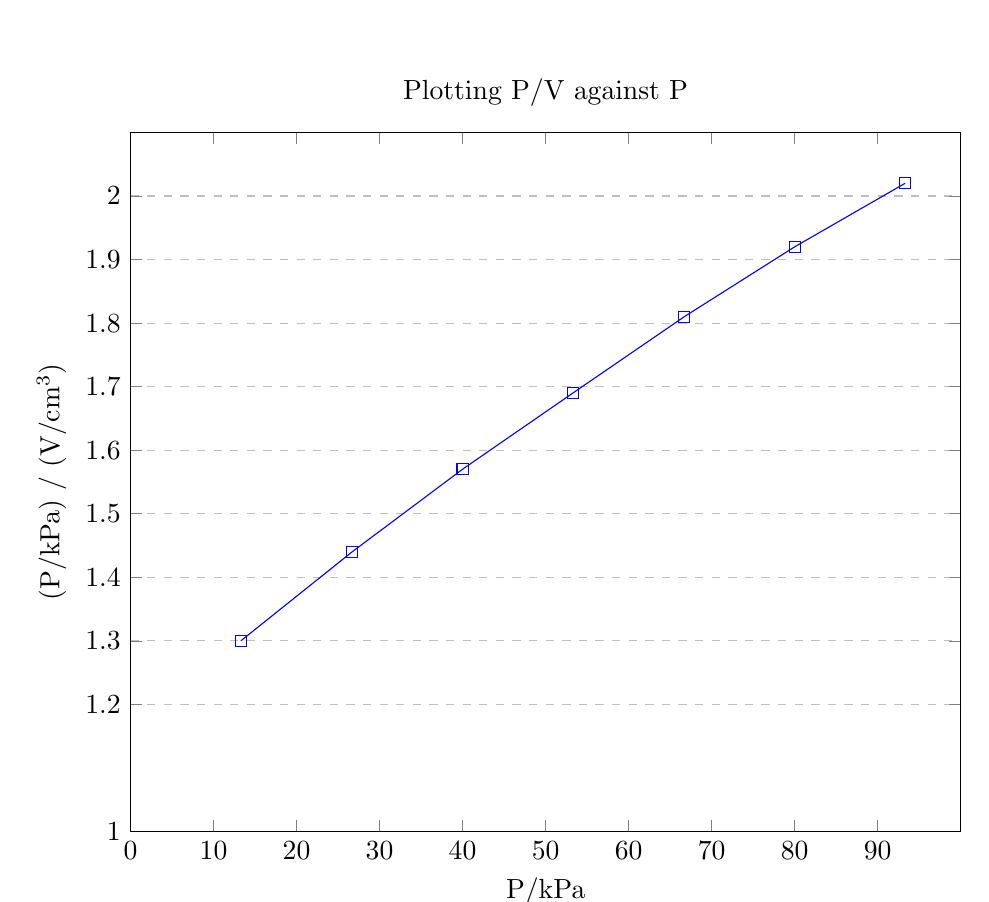
\begin{tikzpicture}
\begin{axis}[
    title={Plotting P/V against P},
    xlabel={P/kPa},
    ylabel={(P/kPa) / (V/cm\(^3\))},
    xmin=0, xmax=100,
    ymin=1, ymax=2.1,
    xtick={0,10,20,30,40,50,60,70,80,90},
    ytick={1,1.2,1.3,1.4,1.5,1.6,1.7,1.8,1.9,2.0},
    legend pos=north west,
    ymajorgrids=true,
    grid style=dashed,
]
 
\addplot[
    color=blue,
    mark=square,
    ]
    coordinates {
    (13.3,1.3)(26.7,1.44)(40.0,1.57)(53.3,1.69)(66.7,1.81)(80.0,1.92)(93.3,2.02)
    };
    %\legend{Linear fit}
 
\end{axis}
\end{tikzpicture}

So the intercept \(\frac{1}{KV_{monolayer}} = 1,20\) and the slope \(\frac{1}{V_{monolayer}} = 111\ cm^3\), \(\therefore K=\frac{1}{111\ cm^3\times 1.20\ kPacm^{-3}} = 7.51 \times 10^{-3}\ kPa^{-1}\)

From the plot we can find the slope of the line, which is equal to 0.0090. The volume of gas required for monolayer coverage is therefore \[V_{monolayer} = 1/0.0090 = 111\ cm^3\]

The intercept for P=0 would be 9.2, so therefore \[K = 1/(111\ cm^3\times 9.2\ Torr\ cm^{-3}) = 0.98\times10^{-3}\ Torr^{-1}\]
\end{example}

\begin{example}{Langmuir Isotherm plotting from data}
Measure the surface coverage at different pressures.

\[\frac{1}{\Theta_e}=1+\frac{1}{KP_A}\]

\begin{tabular}{lc}
\(P_A\) (Torr) & \(\Theta_e\) (273K)\\\hline
0.0 & 0.000\\
10.0 & 0.174\\
20.0 & 0.296\\
30.0 & 0.387\\
40.0 & 0.457\\
50.0 & 0.512\\
60.0 & 0.558\\
70.0 & 0.595\\
80.0 & 0.627\\
90.0 & 0.654\\
100.0 & 0.672\\\hline
\end{tabular}


\begin{tikzpicture}
\begin{axis}[
    title={Plotting \(\Theta_e^{-1}\) vs. \(P_A^{-1}\)},
    xlabel={\(P_A^{-1}\)/Torr},
    ylabel={\(\Theta_e^{-1}\)},
    xmin=0, xmax=0.1,
    ymin=0, ymax=6,
    xtick={0,0.01,0.025,0.04,0.06,0.08,0.1},
    ytick={1,1.5,2,2.5,3,3.5,4,4.5,5,5.5,6},
    legend pos=north west,
    ymajorgrids=true,
    grid style=dashed,
]
 
\addplot[
    color=blue,
    mark=square,
    ]
    coordinates {
    (0.01,1.488)(0.0111,1.529)(0.0125,1.595)(0.0143,1.681)(0.0167,1.792)(0.02,1.953)(0.025,2.188)(0.033,2.584)(0.05,3.379)(0.1,5.747)
    };
    %\legend{Linear fit}
 
\end{axis}
\end{tikzpicture}

From the figure we can see that the slope is: \(\frac{1}{K} = 47.5\) Torr, so \(K=\frac{1}{47.5\ Torr} = 0.0211\ Torr^{-1}\)


When we know the value of K, we can plot the Langmuir isotherm (\(\Theta\) vs. P for given temperature).


\begin{tikzpicture}
\begin{axis}[
    axis lines = left,
    xlabel = P/Torr,
    ylabel = {\(\Theta\)},
    legend pos = south east,
]
%Below the isotherm is defined
\addplot [
    domain=0:1000, 
    samples=100, 
    color=red,
]
{0.0211*x/(1+0.0211*x)};
\addlegendentry{K = 0.0211 Torr\(^{-1}\)}
\end{axis}
\end{tikzpicture}



\end{example}

\subsection{Thermodynamics}

At a given pressure, surface coverage depends on temperature. The constant K is therefore temperature-dependent. let's look out how we can use this fact.

We can rearrange the Langmuir isotherm: 
\[K = \frac{\Theta_e}{P_A(1-\Theta_e)}\]

We can take the logarithm of the equation:
\[lnK = ln\left[\frac{\Theta_e}{(1-\Theta_e)}\right] - ln(P_A)\]

At constant coverage, we can take the partial derivative of the expression with respect to T:

\[\left(\frac{\delta lnK}{\delta T}\right)_\Theta = -\left(\frac{\delta ln(P_A)}{\delta T}\right)_\Theta\]

using the following relationship that we know from Thermodynamics (The Van't Hoff equation): \(\frac{\delta ln K}{\delta T} = \frac{\overline{\Delta H}}{RT^2}\), taking \(\overline{\Delta H}\) to be \(\overline{\Delta H}_{abs}\), we can write:

\[\left(\frac{\delta lnK}{\delta T}\right)_\Theta = - \left(\frac{\delta ln(P_A)}{\delta T}\right)_\Theta = \frac{\overline{\Delta H}_{abs}}{RT^2}\]

Separating and integrating the expression gives us:

\[\int ln(P_A) = - \int \frac{\overline{\Delta H}_{abs}}{RT^2} dT\]

if \(\overline{\Delta H}_{abs}\) is independent of T then

\[ln(P_A) = \left(\frac{\overline{\Delta H}_{abs}}{R}\right)\left(\frac{1}{T}\right) + F(\Theta_e)\] where \(F(\Theta_e)\) is an arbitrary function of equilibrium surface coverage.

Experimentally we can measure \(P_A\) need to maintain constant \(\Theta\) and plot \(ln(P_A\) vs 1/T to get a linear fit with slope equal to \(\frac{\overline{\Delta H}_{abs}}{R}\)

\subsubsection{Enthalpy of Adsorption}
As we saw above, the shape of the isotherm depends on the value of K, and since K is temperature dependent, we can use the isotherm to determine the enthalpy of adsorption.

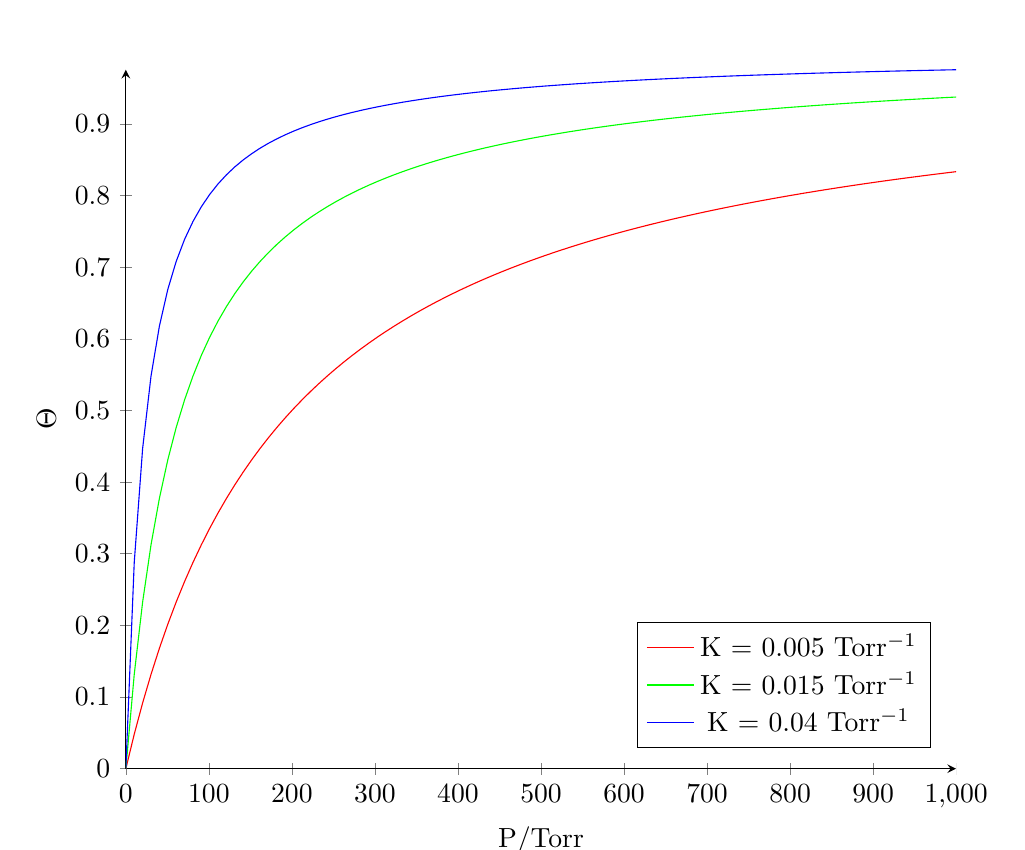
\begin{tikzpicture}
\begin{axis}[
    axis lines = left,
    xlabel = P/Torr,
    ylabel = {\(\Theta\)},
    legend pos = south east,
]
%Below the isotherm is defined
\addplot [
    domain=0:1000, 
    samples=100, 
    color=red,
]
{0.005*x/(1+0.005*x)};
\addlegendentry{K = 0.005 Torr\(^{-1}\)}

%Below the isotherm is defined
\addplot [
    domain=0:1000, 
    samples=100, 
    color=green,
]
{0.015*x/(1+0.015*x)};
\addlegendentry{K = 0.015 Torr\(^{-1}\)}

%Below the isotherm is defined
\addplot [
    domain=0:1000, 
    samples=100, 
    color=blue,
]
{0.04*x/(1+0.04*x)};
\addlegendentry{K = 0.04 Torr\(^{-1}\)}
\end{axis}
\end{tikzpicture}

K can be treated like an equilibrium constant, using the van't Hoff equation:
\[\left(\frac{\delta lnK}{\delta T}\right)_\Theta = \frac{\Delta_{ads}H^\Theta}{RT^2}\]

\begin{example}{Adsorption of CO to a constant coverage}

In an experiment involving adosprion of CO, we'll maintain a constant surface coverage of 10 cm\(^3\) for different temperatures. What is the adsorption enthalpy?

At different temperatures, different pressures are required to maintain the same surface coverage, as in the following table:

\begin{tabular}{lcccccc}
T/K & 200 & 210 & 220 & 230 & 240 & 250\\
P/Torr & 30.0 & 37.1 & 45.2 & 54.0 & 63.5 & 73.9\\
\end{tabular}

From the Langmuir isotherm we have: \(KP = \frac{\Theta}{1-\Theta}\), and for constant surface coverage, \(\Theta\), we also  have: lnK + lnP = constant. Therefore,
\[\left(\frac{\delta lnP}{\delta T}\right)_\Theta = -\left(\frac{\delta lnK}{\delta T}\right)_\Theta = - \frac{\Delta_{ads}H^\Theta}{RT^2}\]

Here we can rewrite the equation using the fact that: \(\left[d\left(\frac{1}{T}\right)dT = -\frac{1}{T^2}\right]\) and we get:

\[\left(\frac{\delta lnP}{\delta (^1/_T)}\right)_\Theta = \frac{\Delta_{ads}H^\Theta}{R}\]

Now we can plot lnP against \(^1/_T\) because the slope of the linear curve fit will be equal to \(\frac{\Delta_{ads}H^\Theta}{R}\)

\begin{tabular}{lcccccc}
T/K & 200 & 210 & 220 & 230 & 240 & 250\\
\(10^3\)/T & 5.0 & 4.76 & 4.55 & 4.35 & 4.17 & 4.00\\
lnP & 3.4 & 3.61 & 3.81 & 3.99 & 4.15 & 4.30\\
\end{tabular}

\begin{tikzpicture}
\begin{axis}[
    title={Plotting lnP vs. \(T^{-1}\)},
    xlabel={\(10^3\)/T},
    ylabel={lnP},
    xmin=4, xmax=5,
    ymin=3.2, ymax=4.5,
    xtick={4.0,4.5,5.0},
    ytick={3.4,3.6,3.8,4.0,4.2},
    legend pos=north east,
    ymajorgrids=true,
    grid style=dashed,
]
 
\addplot[
    color=blue,
    mark=square,
    ]
    coordinates {
    (5.0,3.4)(4.76,3.61)(4.55,3.81)(4.35,3.99)(4.17,4.15)(4.00,4.30)
    };
    %\legend{Linear fit}
\end{axis}
\end{tikzpicture}

We can see the slope is equal to -0.90, so therefore \(\Delta_{ads}H^\Theta = -(0.9\times10^3\ K)\times\ R = -7.5\ kJ\ mol^{-1}\)

\end{example}

\subsubsection{Physisorption and Chemisorption}

Adsorption occurs either as \textit{Physisorption} or \textit{Chemisorption}. \underline{Physisorption} is short for \textit{physical adsorption} and relies on van der waals interactions between the molecule and the surface. The forces act over a relatively long range but they are weak. The energy released upon adsorption is of the same order of magnitude as the enthalpy of condensation. The enthalpy of physisorption can be monitored by the rise in temperature of a sample of known heat capacity and is usually of the order of \(\approx 20\ kJmol^{-1}\). There is no bond breaking. The energy released is not able to make or break bonds, so the molecule is essentially intact, yet not the same as in the gas phase- some perturbations have occurred


\underline{Chemisorption} is short for \textit{chemical adsorption} and occurs when a chemical bond forms between the molecule and the surface. It occurs on sites that maximise their coordination number with surface. The enthalpy of chemisorption is much greater than that of physisorption, of the order of \(\approx 200\ kJmol^{-1}\). A chemisorbed molecule may be fragmented, and this is the reason why solid surfaces \textit{catalyse reactions}. The energy released is able to make or break bonds, so the molecule is altered and is not the same as in the gas phase. Large perturbations have occurred.
 Chemisorption is almost exclusively exothermic, because the translational freedom is reduced since the molecule is immobilised. so in order for the free energy to be negative (\(\Delta G = \Delta H - T\Delta S <0\), it can only be negative if \(\Delta H\) is negative. There are exceptions, such as dissociation of molecule into atoms that move freely on the surface. One example is \ce{H2} adsorbed dissociatively and endothermically because \ce{H2 (g) -> 2H(s)} atoms move freely on surface.

\begin{figure}[H]
\centering
     \begin{subfigure}[b]{0.4\textwidth}
         \centering
         \includegraphics[width=\textwidth]{../../graphics/sorbtion}
         \caption{Activated adsorption}
%         \label{fig:y equals x}
     \end{subfigure}
     \hfill
     \begin{subfigure}[b]{0.55\textwidth}
         \centering
         \includegraphics[width=\textwidth]{../../graphics/nonactivated}
         \caption{Non-activated adsorption}
%         \label{fig:three sin x}
     \end{subfigure}
     \label{fig:activated}
     \caption{The energetics of the adsorption process}
\end{figure}

In activated adsorption (Figure \ref{fig:activated}), there is a potential energy well where the molecule is physisorbed. In order for chemisorption to occur, the molecule has to overcome the energy barrier to move , or activation energy, but in non-actiated adsorption, no additional energy is required to cross between the physisorption well and the chemisorption well

It is also important to consider the \underline{\textit{rate of desorption}}. Desorption is always activated because particles have to be lifted out of a potential well. A physisorbed particle vibrates and might shake itself loose after a time. The temperature dependence of desorption is Arhhenius-like, with an activation energy comparable to the enthalpy of physisorption, \(k_d = Ae^{-\frac{E_d}{RT}}\).

The half-life for remaining on surface has a temperature dependence \(t_{^1/_2} = \frac{ln2}{k_d} = \tau_0e^{\frac{E_d}{RT}}\), where \(\tau_o = \frac{ln2}{A}\)

\subsubsection{Enthalpies of \textit{physisorption} vs enthalpies of \textit{chemisorption}}

Physisorption is a much weaker adsorption than chemisorption. Maximum observed enthalpies of \underline{physisorption} are

\begin{tabular}{lc}
Molecule & \(\Delta_{ads}H^\Theta/(kJmol^{-1})\)\\\hline
\ce{CH4} & -21\\
\ce{H2} & -84\\
\ce{H2O} & -59\\
\ce{N2} & -21\\\hline
\end{tabular}

These enthalpies are insufficient for bond-breaking. The molecule retains its identity on the surface. Due to internal vibrations it can shake itself lose after a period.

Some enthalpies of adsorption for \underline{chemisorption} are:

\begin{tabular}{lccc}
Adsorbate & & Adsorbent & \(\Delta_{ads}H^\Theta/(kJmol^{-1})\)\\\hline
 & Cr & Fe & Ni\\
 \ce{C2H4} & -427 & -285 & -243\\
 CO & & -192 & \\
\ce{H2} & -188 & -134 & \\
 \ce{NH3} & & -188 & -155\\\hline
 \end{tabular}
 
Chemisorbed molecules may be torn apart by unsatisfied valencies of surface atoms

\section{Surface reactions and catalysis}

The reaction between hydrogen and nitrogen to produce ammonia has a very high activation energy. But the reaction can be catalysed by a surface, like Tungsten. This is called heterogeneous catalysis.

\ce{3H2 (g) + N2 (g) ->[W(s)] 2NH3 (g)}

Without a catalyst, the activation energy, \(E_{act}\), is 350 kJmol\(^{-1}\), but with a catalyst it is only 162 kJmol\(^{-1}\).

Another example of a surface catalysed reaction is the production of hydrogen and iodide from hydrogen iodide.

\ce{2HI(g) ->[Au(s) + Pt(s)] H2(g) + I2(g)}

For this reaction, the activation energy is 184 kJmol\(^{-1}\) without the surface and 105 kJmol\(^{-1}\) if it is catalysed by a surface. 

Another example is 

\ce{2N2O (g) ->[Au(s) + Pt(s)] 2N2(g) + O2(g)}

\ce{SO2(g) ->[Pt(s) or V2O5(g)] SO3 (g)}

A very important process in industry is the cracking of high molecular weight hydrocarbons to produce petroleum products, like petrol. This occurs over a mixed catalyst containing \ce{SiO2} and \ce{Al2O3}.

\medskip The activity of a solid catalyst depends on the \underline{physical} and \underline{electronic structure} of the solid and the relationship of the \underline{lattice spacings} to the chemical bonds made or broken during the reaction.

The molar enthalpy of reactants is also very important. If \(|\Delta \overline{H_{ad}}|\) is small, then adsorption is less likely and the rate of reaction will be low.

If \(|\Delta \overline{H_{ad}}|\) is very high then both reactants and products may stay on the surface and the rate of production will be low.

So the effectiveness of a catalyst depends on the adsorption, but also on the physical structure. Increasing the effective surface area increases the effectivenss of a catalyst.

\subsubsection{Adsorption of a single reactant}

A heterogeneous reaction could invlolve just one single reactant species and a surface, e.g. the decomposition of \ce{PH3(g)} on Tungsten at 973 K.

\begin{align*}
A(g) + \otimes \xrightarrow{k_a} \otimes-A &\xrightarrow{k_d} \otimes + A(g)\\
&\xrightarrow{k_r} products\ (F)
\end{align*}

In this situation, the rate of production, R, will be equal to the rate of formation of product:

\(R = \frac{d[F]}{dt} = k_rN\Theta_e\)

\medskip If we assume Langmuir kinetics, we can subsitute the Langmuir isotherm for \(\Theta\), and if we deal with an equilibrium situation with a steady state coverage, \(\Theta_e\), then we can write:

\[\frac{d[F]}{dt} = \frac{k_rNKP_a}{1+KP_A}\]

So the rate of the reaction depends on the pressure of the reactant in the gas phase. For a situation with very low pressure, i.e. \(KP_A << 1\), the expresion reduces to 

\[\frac{d[F]}{dt} \approx k_rNKP_A\]

This is now a first order reaction in A(g). If we have situation with high pressure, i.e. \(KP_A >> 1\), then we get:

\[\frac{d[F]}{dt} = k_rN\]

This is now a zero-order rate law. The next section deals with a situation when we have two reactants.

\subsection{Mechanisms}

For a bimolecular reaction between A and B, catalysed by a surface, we will discuss two different reaction mechanisms, Eley-Rideal and Langmuir-Hinshelwood. The distinction is to do with whether the reaction takes place between two adsorbed molecules \textit{on the surface} or between an adsorbed molecule and a gas-phase molecule. We can have a situation where A adsorbs and reacts with B from the gas phase, or we can have a situation where A and B both adsorb and react \underline{on} the surface.

These mechanisms are the basis of many catalytic processes.

\subsubsection{Eley-Rideal}

The Eley-Rideal mechanism takes place between an adsorbed molecule on the surface and a gas-phase molecule when the gas-phase molecule impacts with the adsorbed molecule, as in the illustration below.

\begin{figure}[H]
\centering
\includegraphics[width=.7\textwidth]{../../graphics/ERmechanism}
\caption{The Eley-Rideal mechanism}
\end{figure}

The reaction rate depends on the \textit{coverage} of the adsorbed species and the \textit{pressure} of the gas-phase species.

It can be described using Langmuir kinetics \(\Theta_A = \frac{k_AP_A}{1+k_AP_A}\) and the overall rate \(= k_{er}\Theta_AP_B\)

\begin{align*}
A(g) \xrightarrow{k_a} \otimes-A &\xrightarrow{k_d} \otimes + A(g)\\
\otimes-A + B(g) &\xrightarrow{k_r} products\ (F)
\end{align*}

In this mechanism the rate of reaction is given by (assuming Langmuir adsorption):

\[\frac{d[F]}{dt} = \frac{k_rK_ANP_BP_A}{1+K_AP_A}\]

because it depends on the coverage of A (from Langmuir isotherm) and pressure of B.

At high pressure, this becomes first order in the gas phase component and zero order in the surface component. At low pressure of adsorbed reactant the reaction is second order.

\begin{align*}
K_AP_A << 1 &\implies \frac{d[F]}{dt} \approx k_rK_ANP_BP_A\\
K_AP_A >> 1 &\implies \frac{d[F]}{dt} \approx k_rNP_B
\end{align*}


\subsubsection{Langmuir-Hinshelwood}

In the Langmuir-Hinshelwood mechanism, the reaction takes place between the two species when they are both adsorbed on the surface. Therefore, it depends on the \underline{coverage of both} species. So both species have to adsorb t become reactive. The product is then desorbed after the reaction. This is important, because if the product didn't desorb it would occupy the surface so the reactant would not be able to adsorb and the reaction could not proceed. Using Langmuir kinetics:

\(\Theta_A = \frac{k_AP_A}{1+k_AP_A}\) and \(\Theta_B = \frac{k_BP_B}{1+k_BP_B}\) and so the overall rate \(= k_{lh}\Theta_A\Theta_B\)

\begin{figure}[H]
\centering
\includegraphics[width=.7\textwidth]{../../graphics/LHmechanism}
\caption{The Langmuir-Hinshelwood mechanism}
\end{figure}

How do we get this? The Langmuir isotherm applied to both reactants will give us:

\begin{align*}
A(g) + \otimes &\xrightarrow{k_a} \otimes-A \xrightarrow{k_d} \otimes + A(g)\\
B(g) + \otimes &\xrightarrow{k_b} \otimes-B \xrightarrow{k_{db}} \otimes + B(g)\\
\otimes-A + \otimes-B &\xrightarrow{k_r} products\ (F)
\end{align*}

The rate of reaction now depends on the surface coverage of \textit{both} species:

\[ \frac{d[F]}{dt} = k_r(N\Theta_e^A)(N\Theta_e^B)\]

So substituting for \(\Theta\) we get:

\[ \frac{d[F]}{dt} = \frac{k_rN^2K_AK_BP_AP_B}{(1+K_AP_A + K_BP_B)^2}\]

At low partial pressures of A and B we get a simple second order rate law: \(R \approx k_rN^2K_BK_AP_AP_B\)

At high pressures, no simple rate law describes the kinetics. If \(P_A >> P_B\) or vice versa, the reaction rate will be very slow.
(\textbf{EXERCISE: show why this is the case})

\part{Analytical methods}

\section{Ultrahigh Vacuum Systems}
Due to high collision rate at pressures even as low as \(10^{-6}\) Torr, surface analysis requires ultrahigh vacuum (UHV) in order to keep the surface clean for long enough to study it. Ultrahigh vacuum systems are usually of stainless steel construction (to withstand the atmospheric pressure), and in order to bring doen the pressure inside them, typically three types of pumps ar eemployed. A \textit{rotary vane pump} will acieve a vacuum of around \(10^{-3}\) Torr, a \textit{diffustion} or \textit{turbo molecular pump} will bring the vacuum down further to \(10^{-8}\) Torr, and an \textit{ion} or \textit{sublimation pump} will acieve a vacuum of \(10^{-10}\) Torr or lower. Sample handling in such a system therefore requires mechanical sample transfer arms, and such systems usually include heating and cooling stages, ion bombardment for sample cleaning, and in-situ surface analysis techniques.

\begin{center}\includegraphics[width=.7\textwidth]{../../graphics/uhv}\end{center}

The figure shows a typical UHV system for surface analysis

\section{Temperature Programmed Desorption}

There are many techniques which use \textit{temperature-programming} to discriminate between processes with different activation parameters. For single crystal studies, a very useful techique is \textit{Temperature Programmed Desorption}, or TPD.

When the technique is applied to a system in which the adsorption process is, at least in part, irreversible and T-programming leads to surface reactions, then this technique is often known as \textit{Temperature Programmed Reaction Spectroscopy}, or TPRS.

The technique usually involves:
\begin{enumerate}
\item Adsorption of one or more molecular species onto the sample surface at low temperature (frequently 300 K, but sometimes sub-ambient)
\item Heating of the sample in a controlled manner (preferrably so as to give a linear temperature ramp) whilts monitoring the evolution of species from the surface back into the gas phase
\end{enumerate}

\includegraphics[width=\textwidth]{../../graphics/tpd1}

Note that continuous pumping is required. Without pumping we will get a graph like the one on the left, but with pumping we will see a peak like the one on the right. The location and intensitoy of the peak gives us the information we want.

The monitoring of the gas phase can be done in several different ways. Merely monitoring the change in pressure will give us the location of the peak, which tells us what temperature the adsorbed species desorb at. But if we have multiple different species on the surface, or a mixture of reaction products, then we can keep an eye on each one using a \underline{mass spectrometer}, which allows us to monitor several gas-phase species simultanelously.

\begin{center}\includegraphics[width=\textwidth]{../../graphics/tpd2}\end{center}

The illustration shows a situation with a crystal surface in a vacuum chamber, with a linear temperature ramp. The species evolving from the surface are monitored with a mass spectrometer. The mass spectrometer requires vacuum to operate, which is an other reason why we need UHV. The mass spectrometer also lets us check for leaks in the vacuum system, because we can look for air components like \ce{O2} and \ce{N2} in the signal. Many systems have a mass spectrometer for this specific purpose anyway.

\medskip An experiment typically involves recording the intensity of the signal (pressure and/or mass spectrometry signal) over time, as the temperature changes in a well-controlled manner according to the temperature program, \textit{so we can convert the time axis to a temperature axis}.

\begin{center}\includegraphics[width=.6\textwidth]{../../graphics/tpd3}\end{center}

The graph above shows data from a TPD experiment following adsorption of CO onto a Pd(111) crystal at 300 K. There is one desorption peak at T > 300 K.

\begin{center}\includegraphics[width=.6\textwidth]{../../graphics/tpd4}\end{center}

The graph above shows another example, involving the adsorption of oxygen on Pd(111) at 80 K. Under these conditions, \ce{O2} forms two distinct adsorbed states -- one strongly bound and one much more weakly bound. The strongly bound species desorbs at the higher temperature (broad peak), whereas the weakly bound form desorbs almost immediately.

Some important points:

\begin{itemize}
\item The area under the peak is proportional to the amount originally adsorbed, i.e. proportional to the surface coverage
\item The kinetics of desorption (obtained from the peak profile and the coverage dependence of the desorption characteristics) give information on the state of aggregation of the adsorbed species, e.g. molecular vs. dissociative
\item The position of the peak (the \textit{peak temperature}) is related to the enthalpy of adsorption, i.e. to the strength of binding to the surface
\end{itemize}

Let's consider an elementary first order desorption reaction: \ce{A(ads) -> A (g)}

Let the concentration of coverage of A be called \(\Theta\), as before, let the rate constant for the desorption reaction be \(k\), as usual.

The signal (intensity, or counts per second), I(t), measured by the mass spectrometer at any time, t, will be proportional to the \textit{rate of change} of coverage:

\begin{center}\colorbox{cyan}{\textcolor{black}{\(I(t) \propto -\frac{d\Theta}{dt}=k\Theta^x\)}}\end{center}

where x is the order of reaction. In the following, we will assume first order reaction, so x = 1.

From Arrhenius theory, we have the expression \(k = Ae^{\frac{-E_a}{RT}}\), where A is the pre-exponential factor and \(E_a\) is the activation energy for desorption. That means we can write:
\begin{equation}\label{roc} I(t) \propto - \frac{d\Theta}{dt} = A\Theta e^{-\frac{E_a}{RT}}\end{equation}

This gives the rate of change of intensity and rate of change of coverage as a function of time, t. Now we can convert this to rate of change of coverage with respect to T, because we have a linear temperature ramp, i.e. the temperature changes linearly with time:

\(T(t) = T_0 + \beta t\), where \(\beta\) is the heating rate, \(\frac{dT}{dt}\)

since \(\beta = \frac{dT}{dt}\) and \(\frac{d\Theta}{dt} = \left(\frac{d\Theta}{dT}\right)\left(\frac{dT}{dt}\right)\) we can write:

\[\frac{d\Theta}{dt} = \frac{d\Theta}{dT} \times \beta\]
in other words, \(-\frac{d\Theta}{dT} = -\frac{d\Theta}{dt} \frac{1}{\beta}\). Combining this with equation \ref{roc}, we get:

\begin{equation}
\boxed{-\frac{d\Theta}{dT} =I(T) =  A\frac{\Theta}{\beta}e^{-^{E_a}_{RT}}}
\end{equation}

Now we have an expression for the rate of change of coverage, and signal intensity, with temperature. Equation \ref{roc} is called the \textit{Polyani-Wigner} equation.

Note that at the peak temperature (red arrow in the graph above), the rate of change is zero, i.e. \(\frac{dI(T)}{dt}=0\).

We must evaluate the differential \(\frac{dI(T)}{dt}\). In other words, we have to evaluate:
\[\frac{d\left[A\frac{\Theta}{\beta}e^{-^{E_a}/_{RT}}\right]}{dT} = 0\]

But we must remember that equilibrium coverage, \(\Theta_e\), also depends on temperature, \(\Theta(T)\), so the expression to evaluate is:

\begin{equation}\label{dit} \frac{d\left[A\frac{\Theta(T)}{\beta}e^{-^{E_a}/_{RT}}\right]}{dT} = 0\end{equation}

This is called \underline{redhead Analysis}. In order to get the derivative of the expression \ref{dit} we employ the derivation rule: (uv)' = u'v + uv'. So

\[\frac{dI(T)}{dT} = \frac{d\Theta}{dT}\left[\frac{A}{\beta}e^{-^{E_a}/_{RT}}\right]+\frac{\Theta A}{\beta}\frac{E_a}{RT^2}e^{-^{E_a}/_{RT}}=0\]

But we have also seen that \(\frac{d\Theta}{dT} = -A\frac{\Theta}{\beta}e^{-^{E_a}/_{RT}}\), so we can write:

\begin{equation}\label{prered} -A\frac{\Theta}{\beta}e^{-^{E_a}/_{RT}}\left[\frac{A}{\beta}e^{-^{E_a}/_{RT}}\right]+\frac{\Theta A}{\beta}\frac{E_a}{RT^2}e^{-^{E_a}/_{RT}}=0\end{equation}

We can start simplifying equation \ref{prered} by removing common factors. First, we can divide through by A. Then we can divide through by \(\Theta\). We can do this because we said that we assumed first order reaction, x=1, so there is no coverage dependence. Next, we can divide through by \(\frac{1}{\beta}\), and then we divide through by \(e^{-^{E_a}/_{RT}}\). Then we multiply up by \(\beta\) and divide through by \(\frac{E_a}{R}\), then multiply by -1 (\textbf{EXERCISE: try this yourself}). Now we are left with the expression:
\[\frac{RA}{E_a}e^{-^{E_a}/_{RT}} - \frac{\beta}{T^2} = 0\]
If we take the logarithm of the last expression
\[ln\left(\frac{RA}{E_a}\right) - \frac{E_a}{RT} - ln\left(\frac{\beta}{T^2}\right) = 0\]
and rearrange (remember: \(ln\left(\frac{x}{y}\right) = -ln\left(\frac{y}{x}\right)\)
\begin{equation}\label{redhead}
\boxed{ln\left(\frac{T^2}{\beta}\right) = \frac{E_a}{RT} - ln\left(\frac{RA}{E_a}\right)}
\end{equation}

This equation (\ref{redhead}) is the result we need. Now we can plot \(ln\left(\frac{T^2}{\beta}\right)\) vs \(\frac{1}{T}\) and we'll get a linear graph with a slopw given by \(\frac{E_a}{R}\) and an intercept equal to \(-ln\left(\frac{RA}{E_a}\right)\). The temperature T in the expression is the peak temperature associated with heating rate \(\beta\).

\begin{example}{Data Trreatment}

The following data were obtained from a series of temperature programmed desorption (TPD) experiments aimed at studying the desorption of molecular benzene from a metal surface:
Assuming that the desorption process may be described by first order kinetics, determine the activation energy of desorption.

\begin{tabular}{lccccc}
Peak desorption temperature (K) & 300 & 295 & 293 & 287 & 283\\
heating rate (\(Ks^{-1}\)) & 20 & 15 & 9 & 5 & 3
\end{tabular}

To determine the activation energy, we have to find the slope of the line we get from plotting \(ln\left(\frac{T^2}{\beta}\right)\) vs \(\frac{1}{T}\). So first we have to do some calculations:

\begin{tabular}{lccccc}
Peak T (K) & \(\beta\ (Ks^{-1})\) & \(T^2\) & \(T^2/\beta\) & ln\((T^2/\beta)\) & 1/T\\\hline
300 & 20 & 90000 & 4500 & 8.412 & 0.00333\\
295 & 15 & 87025 & 5801.67 & 8.666 & 0.00339\\
293 & 9 & 85849 & 9538.78 & 9.163 & 0.00341\\
287 & 5 & 82369 & 16473.8 & 9.710 & 0.00348\\
283 & 3 & 80089 & 26696.33 & 10.192 & 0.00353\\\hline
\end{tabular}

Now, plotting the points, we get:

\begin{tikzpicture}
\begin{axis}[
    title={Plotting \(ln\left(\frac{T^2}{\beta}\right)\) vs \(\frac{1}{T}\)},
    xlabel={1/T},
    ylabel={ln\((T^2/\beta)\)},
    xmin=0.0033, xmax=0.00355,
    ymin=7, ymax=10.5,
 %   xtick={4.0,4.5,5.0},
 %   ytick={3.4,3.6,3.8,4.0,4.2},
    legend pos=north east,
    ymajorgrids=true,
    grid style=dashed,
]
 
\addplot[
    only marks,
    color=blue,
    mark=square,
    ]
    coordinates {
    (0.00333,8.411)(0.00339,8.666)(0.00341,9.163)(0.00348,9.7095)(0.00353,10.192)
    };
    %\legend{Linear fit}
\end{axis}
\end{tikzpicture}

A stright line fit of the points in the graph would have a slope equal to 9172.8, which is equal to \(E_a/R\). That gives us a value for \(E_a\) of 76.27 kJmol\(^{-1}\). That is the activation energy we were looking for.

\end{example}

\subsection{zero, first and second order reactions}

The figure below shows a \underline{simulated first order TPD experiment}: Consider a first order reaction between adsorbates and surface. Values of the peak temperature, \(T_m\) are constant as the initial coverage \(\Theta\) varies from \(1.0 \times 10^{13}\) to \(6.0 \times 10^{13}\ cm^{-2}\). \(E_a = 30\) kJ/mol, \(\beta = 1.5^\circ C/s,\ A = 1 \times 10^{13}\ s^{-1}\). 

\includegraphics[width=\textwidth]{../../graphics/tpd1st}

\textbf{Note that the peak position does not change with coverage}, because for first order the interaction to consider is simply that between the adsorbate and the surface.

The next figure shows a \underline{simulated second-order TPD experiment}: Now there is a second-order reaction between adsorbates and surface. Values of \(T_m\) decrease as the initial coverage \(\Theta\) increases from \(1.0 \times 10^{13}\) to \(6.0 \times 10^{13}\ cm^{-2},\ E_a = 30\) kJ/mol, \(\beta = 1.5^\circ C/s,\ A = 1 \times 10^{-1}\).

\includegraphics[width=\textwidth]{../../graphics/tpd2nd}

\textbf{Note that the peak position shifts to lower T as initial coverage increases}, because for second order the interactions to consider are now those between adsorbed species as well as those between the adsorbate and the surface.

The next figure shows a \underline{simulated zero-order TPD experiment}: A zero-order reaction between adsorbates and surface. Values of \(T_m\) increase apparently as the initial coverage \(\Theta\) increases from \(1.0 \times 10^{13}\) to \(6.0 \times 10^{13}\ cm^{-2},\ E_a = 30\) kJ/mol, \(\beta = 1.5^\circ C/s,\ A = 1 \times 10^{28}\).

\includegraphics[width=\textwidth]{../../graphics/tpdzero}

\underline{Note that all the features have the same leading edge}. This is because for zeroth order the system is essentially one where multilayers of material have condensed onto the surface. The energy required to remove any molecule in a multilayer is essentially independent of the layer thickness

\medskip The important thing is that we can get \(E_a\), A and the order from the experimental TPD data.

\begin{figure}[H]
\centering
Example of a second order desorption experiment

\includegraphics[width=.6\textwidth]{../../graphics/tpdexp}
\caption{Adsorption–desorption of \ce{O2} from an amorphous silicate surface kept at 20 K for different coverages. The heating ramp rate during the TPD stage is about 1 K/s. Note the shift of the peak to lower T as \(\Theta\) increases}
\end{figure}

\section{Electron spectroscopy}

What happens on a surface? The figure illustrates a couple of possibilities when formic acid and hydrazine are adsorbed on a Copper (110) surface. They can adsorb side by side or they can be stacked. Do they undergo any reactions? How can we find out?

\begin{center}\includegraphics[width=.5\textwidth]{../../graphics/formiconCu}\end{center}

We can try using quantum mechanical modelling. The next figure shows the two situations as a computer model sees it.

\begin{figure}[H]
\centering
\begin{subfigure}[t]{.4\textwidth}
\includegraphics[width=\textwidth]{../../graphics/formiconcucalc1}
\caption{Calculated adsorption geometry for formic acid and hydrazine coadsorbed side-by
side on a Cu(110) surface.}
\end{subfigure}
\begin{subfigure}[t]{.4\textwidth}
\includegraphics[width=\textwidth]{../../graphics/formiconcucalc2}
\caption{Calculated adsorption geometry for formic acid and hydrazine coadsorbed on a
Cu(110) surface, with formic acid bonded on top of the adsorbed hydrazine. }
\end{subfigure}
\caption{Computer model views of adsorption of formic acid and hydrazine on Copper (110)}
\end{figure}

But we also need a way of experimentally ``seeing'' what is happening on the surface at a molecular level. Electron spectroscopy methods allow us to probe the bonding and molecular structure of atoms and molecules on a surface.

\subsection{X-ray Photoelectron Spectroscopy (XPS)}

XPS is also known as Electron Spectroscopy for Chemical Analysis (ESCA). In this technique, X-rays are employed to impart energy on core level electrons leading to their ejection from the material surface. The primary event in this technique is the ejection of a photoelectron.

\begin{center}\includegraphics[width=.6\textwidth]{../../graphics/electronspectroscopy}\end{center}

\includegraphics[width=\textwidth]{../../graphics/xps1}

\subsubsection{Binding Energies}

The important information that XPS provides is the \textit{\underline{binding energies}} of the electrons that are ejected. These are calculated from the following equation:

\begin{equation}
E_k = h\nu - E_B - \phi_s
\end{equation}

\begin{figure}
\centering
\includegraphics[width=.6\textwidth]{../../graphics/photoemission}
\caption{in XPS, incoming X-rays lead to ejection of a core electron. The kinetic energy of the electron is measured and from this its binding energy is known}
\end{figure}

\begin{figure}
\centering
\includegraphics[width=.6\textwidth]{../../graphics/xps2}
\caption{Illustration of the steps involved in the XPS technique}
\end{figure}

\begin{figure}
\centering
Typical XPS scan, Ru single crystal surface

\includegraphics[width=.6\textwidth]{../../graphics/xps3}
\caption{Not the use of binding energies with distinct peaks for certain binding energies providing information on the chemical species on the surface. Also not the appearance of ``Auger'' peaks (more of which below)}
\end{figure}

The electrons' \underline{Binding energies} are dependent on the atomic number, the shell and the chemcial environment. This figure illustrates how the binding energies depend on atomic number and shell

\begin{center}\includegraphics[width=.7\textwidth]{../../graphics/bindingenergies}\end{center}

The following experiment illustrates the power of the technique. A Copper(110) surface is exposed to gas phase formic acid and hydrazine. The exposure is measured in Langmuirs (L). The experiments compare what happens when the clean Cu surface is exposed to formic acid first, then hydrazine, or when the clean surface is exposed to hydrazine first, then formic acid. The example is taken from Yao et al. J. Phys. Chem. C, 2019, DOI: 10.1021/acs.jpcc.8b01804.

\begin{center}\includegraphics[width=.7\textwidth]{../../graphics/xpsexp1}\end{center}

The figure shows  X-ray photoelectron spectroscopy (XPS) data for 20 L of N2H4 + 20 L of HCOOH adsorbed sequentially on a Cu(110) surface. Results are shown as a function of annealing  temperature.  The signal intensities shown are the binding energies relating to C 1s (left panel), O 1s (center), and N 1s (right). Reference traces are also provided at the bottom for the clean surface and for 10 L of HCOOH or 20 L of N2H4 adsorbed alone on the clean Cu(110).

%Discuss observations here

We see in the figure above that there are XPS spectra for different tempoeratures in the same experiment. So it is possible to study the Temperature Programmed Desorption simultanelously. This is shown in the next figure

\begin{center}\includegraphics[width=.9\textwidth]{../../graphics/xpsexp2}\end{center}

The figure compares TPD results with formic acid and hydrazine coadsorbed on Cu(110) at 150 K as a function of the order of dosing. Traces for each of the two reactants when adsorbed alone, by themselves, are provided as well for reference. The data correspond to the desorption of (from left to right): \ce{H2} (2 amu), \ce{NH3} (17 amu), \ce{N2} (28 amu, after deconvolution of the \ce{N2H4} and \ce{CO2} contributions), \ce{N2H4} (29 amu), \ce{CO2} (44 amu), and \ce{HCOOH} (46 amu). 3.0 L exposures were used in all cases.

%Discuss figure here

\subsubsection{Surface coverage from XPS}

The XPS technique provides a direct measure of the relative surface abundances of different atomic elements. This enables us to determine surface coverage as well.

\begin{center}\includegraphics[width=.9\textwidth]{../../graphics/xpsexp3}\end{center}

The figure shows C, O, and N atomic surface coverages on Cu(110) as a function of annealing temperature for Cu(110) dosed sequentially with 20 L of \ce{N2H4} + 20 L of \ce{HCOOH}, estimated from the XPS peak areas after proper calibration

\subsubsection{Why is the technique surface sensitive?}

The X-rays can penetrate the surface to a depth of 1 \(\mu m\), so why does it only give us information about the surface to a depth of about 10 nm?

\begin{center}\includegraphics[width=.8\textwidth]{../../graphics/xps4}\end{center}

The reason is that the electrons ejected from their core shelss can only escape from the solid if they are very close to the surface. That is related to the \textit{inelastic mean free path}, i.e. the mean distance an electron can travel without being scattered. 

\begin{figure}[H]
\centering
\begin{subfigure}[b]{.45\textwidth}
\includegraphics[width=\textwidth]{../../graphics/meanfreepath}
\end{subfigure}
\begin{subfigure}[b]{.45\textwidth}
\includegraphics[width=\textwidth]{../../graphics/meanfreepath2}
\end{subfigure}
\caption{Mean free path (MFP)  = average distance travelled by the electron before undergoing a scattering event, so only photoelectrons created near to the surface can escape into the vacuum}
\end{figure}

\subsubsection{Chemical shifts in XPS}

\begin{figure}[H]
\centering
\begin{subfigure}[b]{.45\textwidth}
\includegraphics[width=\textwidth]{../../graphics/chemshift1}
\end{subfigure}
\begin{subfigure}[b]{.45\textwidth}
\includegraphics[width=\textwidth]{../../graphics/chemshift2}
\end{subfigure}
\caption{Rough ‘rule of thumb’: between 1 and 2 eV shift for every unit change of oxidation state}
\end{figure}

\begin{figure}[H]
\centering
\begin{subfigure}[b]{.45\textwidth}
\includegraphics[width=\textwidth]{../../graphics/chemshift3}
\end{subfigure}
\begin{subfigure}[b]{.45\textwidth}
\includegraphics[width=\textwidth]{../../graphics/chemshift4}
\end{subfigure}
\caption{}
\end{figure}

\subsection{Auger Electron Spectroscopy}

\begin{center}\includegraphics[width=.8\textwidth]{../../graphics/xps5}\end{center}

As well as the primary event, which is the ejection of an electron from its core shell into the vacuum, there are secondary events, which are ejctions of ``Auger'' electrons, due to energy released when higher level electrons fill vacancies left behind by core shell electrons.

\subsection{Ultraviolet Photoelectron Spectroscopy (UPS)}

\begin{center}\includegraphics[width=.8\textwidth]{../../graphics/uvs}\end{center}

\underline{Example of UPS in action: characterisation of CO bonding on Copper and Nickel surfaces}

\begin{center}\includegraphics[width=.8\textwidth]{../../graphics/ups2}\end{center}

The figure shows a molecular orbital diagram of gas-phase carbon monoxide. 
Note lone pairs: 4s on oxygen and 5s on carbon

\begin{center}\includegraphics[width=.8\textwidth]{../../graphics/ups3}\end{center}

The figure shows a gas-phase UPS spectra from carbon monoxide.
What are the splittings of the features shown?

\begin{figure}[H]
\centering
\begin{subfigure}[b]{.45\textwidth}
\includegraphics[width=\textwidth]{../../graphics/ups4}
\caption{UPS data showing the real density of states for these metals}
\end{subfigure}
\begin{subfigure}[b]{.45\textwidth}
\includegraphics[width=\textwidth]{../../graphics/ups5}
\caption{density of states for the 4s and 3d electrons of both Ni and Cu}
\end{subfigure}
\caption{Note the position of the Fermi Level in both cases. The Fermi level will influence reactivity.........but how?}
\end{figure}

\begin{figure}[H]
\centering
\begin{subfigure}[b]{.45\textwidth}
\includegraphics[width=\textwidth]{../../graphics/ups6}
\caption{UPS data for CO on Cu at 20K. Note the similarity between the surface  spectrum and the gas phase spectrum}
\end{subfigure}
\begin{subfigure}[b]{.45\textwidth}
\includegraphics[width=\textwidth]{../../graphics/ups7}
\caption{UPS data for CO on Ni at 300K. Note the differences  between the surface  spectrum and the gas phase spectrum}
\end{subfigure}
\caption{Note that the metal bands also yield UPS data}
\end{figure}


\begin{frame}
\end{frame}

\end{document}

